% =============================================================================
% Chapter 3: League Game - Multi-Agent Architecture
% מערכת הליגה - ארכיטקטורה רב-סוכנית
% Based on original Chapter 6
% =============================================================================

\documentclass[../master/main.tex]{subfiles}

\begin{document}

\setcounter{chapter}{2}
\hebrewchapter{מערכת הליגה --- ארכיטקטורה רב-סוכנית}
\hebrewchapterlabel{chap:architecture}

\hebrewsection{מבוא}

פרק זה מציג את הארכיטקטורה המודולרית של מערכת הליגה. המערכת מבוססת על הפרדה ברורה בין שכבות התפעול השונות, מה שמאפשר גמישות, תחזוקה קלה, ויכולת להחליף את חוקי המשחק מבלי לשנות את הפרוטוקול.

\hebrewsubsection{מטרות הפרק}

בסיום פרק זה, תבינו:
\begin{itemize}
    \item את עקרון ההפרדה לשלוש שכבות: ליגה, שיפוט וחוקי משחק
    \item את שלושת סוגי הסוכנים: מנהל ליגה, שופט ושחקן
    \item את מכונות המצבים של כל סוכן
    \item את מנגנון הזהויות (\en{IDs}) והמעקב
    \item את מערכת הניקוד המפורטת
\end{itemize}

% =============================================================================
\hebrewsection{ארכיטקטורת שלוש שכבות}
\label{sec:three-layers}
% =============================================================================

\hebrewsubsection{עקרונות התכנון}

המערכת תוכננה על פי מספר עקרונות מנחים:

\begin{enumerate}
    \item \textbf{עצמאות שפת תכנות} --- כל סטודנט יכול לממש סוכן בשפה לבחירתו
    \item \textbf{הפרדת אחריות} --- כל סוכן אחראי לתפקיד מוגדר בלבד
    \item \textbf{פרוטוקול פתוח} --- הודעות במבנה \en{JSON} עם שדות חובה ורשות
    \item \textbf{מקור אמת יחיד} --- השופט הוא מקור האמת למצב המשחק
\end{enumerate}

\hebrewsubsection{תרשים שלוש השכבות}

איור~\ref{fig:three-layers-arch} מציג את ארכיטקטורת שלוש השכבות.

\begin{figure}[htbp]
\centering
\begin{english}
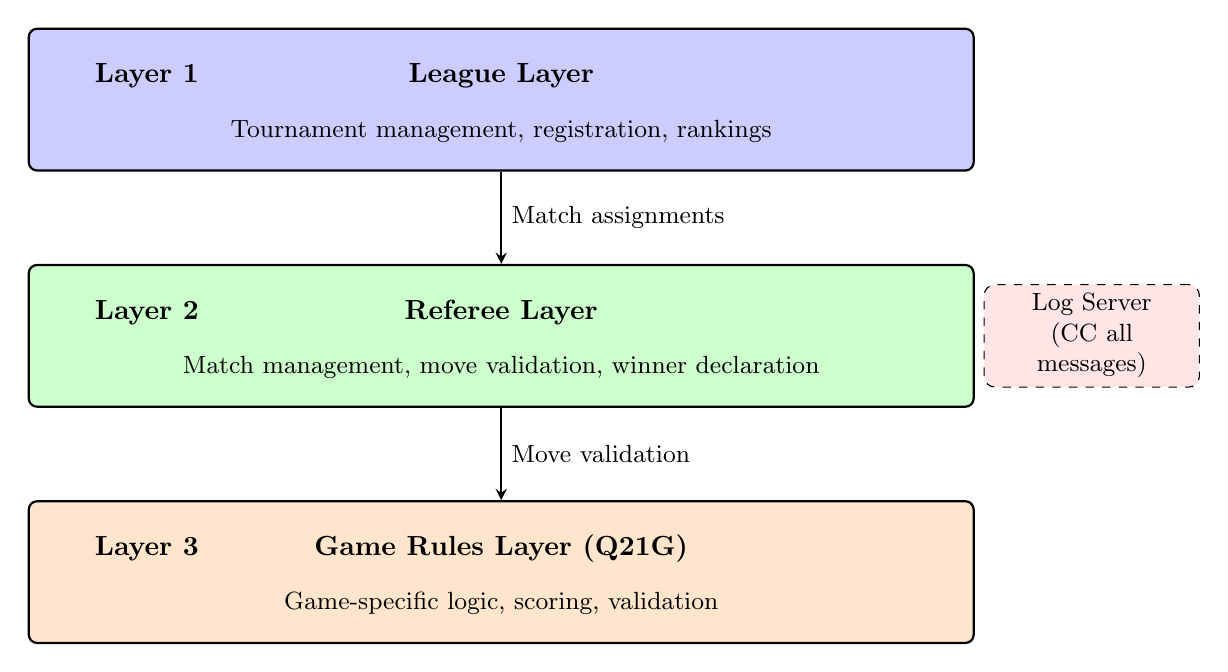
\begin{tikzpicture}[
    layer/.style={draw, thick, fill=#1!20, minimum width=12cm, minimum height=1.8cm, rounded corners=3pt},
    label/.style={font=\bfseries},
    arrow/.style={->, thick, >=stealth}
]
    % Layer 1 - League
    \node[layer=blue] (league) at (0,6) {};
    \node[label] at (-4.5,6.3) {Layer 1};
    \node at (0,6.3) {\textbf{League Layer}};
    \node[font=\small] at (0,5.6) {Tournament management, registration, rankings};

    % Layer 2 - Referee
    \node[layer=green] (referee) at (0,3) {};
    \node[label] at (-4.5,3.3) {Layer 2};
    \node at (0,3.3) {\textbf{Referee Layer}};
    \node[font=\small] at (0,2.6) {Match management, move validation, winner declaration};

    % Layer 3 - Game Rules
    \node[layer=orange] (rules) at (0,0) {};
    \node[label] at (-4.5,0.3) {Layer 3};
    \node at (0,0.3) {\textbf{Game Rules Layer (Q21G)}};
    \node[font=\small] at (0,-0.4) {Game-specific logic, scoring, validation};

    % Arrows
    \draw[arrow] (league.south) -- (referee.north) node[midway, right, font=\small] {Match assignments};
    \draw[arrow] (referee.south) -- (rules.north) node[midway, right, font=\small] {Move validation};

    % Side note - Log Server
    \node[draw, dashed, fill=red!10, rounded corners, text width=2.5cm, align=center, font=\small] at (7.5,3) {Log Server\\(CC all messages)};
\end{tikzpicture}
\end{english}
\caption{ארכיטקטורת שלוש השכבות עם שרת הלוג}
\label{fig:three-layers-arch}
\end{figure}

\hebrewsubsection{שכבה ראשונה: ניהול הליגה}

שכבת הליגה (\en{League Layer}) אחראית על:

\begin{itemize}
    \item \textbf{רישום שחקנים ושופטים} --- קליטה והקצאת מזהים ייחודיים
    \item \textbf{יצירת לוח משחקים} --- הקצאת שלישיות לכל מחזור
    \item \textbf{ניהול דירוג} --- חישוב ופרסום טבלת הדירוג
    \item \textbf{שידורים} --- הודעות כלליות לכל המשתתפים
\end{itemize}

\hebrewsubsection{שכבה שנייה: שיפוט משחקים}

שכבת השיפוט (\en{Referee Layer}) מנהלת משחקים בודדים:

\begin{itemize}
    \item \textbf{תיאום הגעה} --- הזמנת שחקנים וקבלת אישור
    \item \textbf{ניהול שלבי המשחק} --- מעבר בין השלבים השונים
    \item \textbf{חישוב ציונים} --- הערכת הניחושים ומתן משוב
    \item \textbf{דיווח לליגה} --- שליחת תוצאות למנהל הליגה
\end{itemize}

\hebrewsubsection{שכבה שלישית: חוקי המשחק}

שכבת חוקי המשחק (\en{Game Rules Layer}) מכילה את הלוגיקה של \en{Q21G}:

\begin{itemize}
    \item \textbf{בחירת פסקה} --- בחירה מחומרי ההרצאות
    \item \textbf{יצירת רמזים} --- כותרת, תיאור, אסוציאציה
    \item \textbf{אימות תשובות} --- בדיקת שאלות ותשובות
    \item \textbf{חישוב ציון} --- ארבעת הרכיבים
\end{itemize}

% =============================================================================
\hebrewsection{סוגי הסוכנים}
\label{sec:agent-types}
% =============================================================================

\hebrewsubsection{תרשים אינטראקציה}

איור~\ref{fig:agent-interaction-arch} מציג את התקשורת בין הסוכנים, כולל זרימת שידורים.

\begin{figure}[htbp]
\centering
\begin{english}
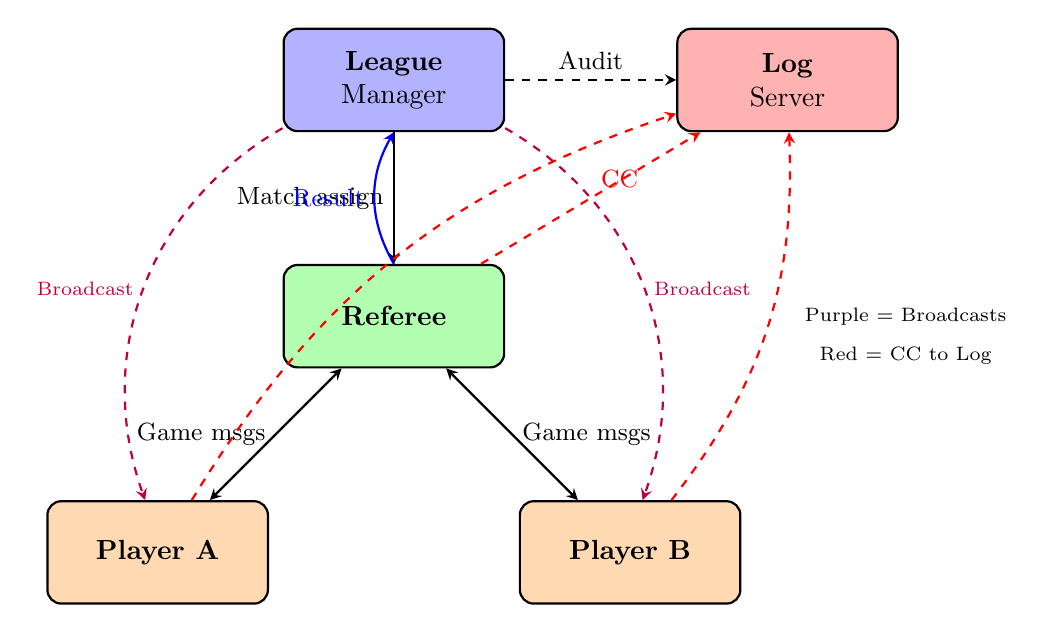
\begin{tikzpicture}[
    agent/.style={draw, thick, fill=#1!30, minimum width=2.8cm, minimum height=1.3cm, rounded corners=5pt, align=center},
    arrow/.style={->, thick, >=stealth},
    bidir/.style={<->, thick, >=stealth},
    broadcast/.style={->, thick, >=stealth, purple, dashed}
]
    % Agents
    \node[agent=blue] (manager) at (0,4) {\textbf{League}\\Manager};
    \node[agent=red] (log) at (5,4) {\textbf{Log}\\Server};
    \node[agent=green] (referee) at (0,1) {\textbf{Referee}};
    \node[agent=orange] (p1) at (-3,-2) {\textbf{Player A}};
    \node[agent=orange] (p2) at (3,-2) {\textbf{Player B}};

    % Manager connections
    \draw[arrow] (manager) -- (referee) node[midway, left, font=\small] {Match assign};
    \draw[arrow, dashed] (manager) -- (log) node[midway, above, font=\small] {Audit};

    % Broadcast arrows (purple dashed)
    \draw[broadcast] (manager) to[bend right=40] node[midway, left, font=\scriptsize, purple] {Broadcast} (p1);
    \draw[broadcast] (manager) to[bend left=40] node[midway, right, font=\scriptsize, purple] {Broadcast} (p2);

    % Referee connections
    \draw[bidir] (referee) -- (p1) node[midway, left, font=\small] {Game msgs};
    \draw[bidir] (referee) -- (p2) node[midway, right, font=\small] {Game msgs};

    % CC to log
    \draw[arrow, dashed, red] (referee) -- (log) node[midway, above right, font=\small] {CC};
    \draw[arrow, dashed, red] (p1) to[bend left=20] (log);
    \draw[arrow, dashed, red] (p2) to[bend right=20] (log);

    % Result back
    \draw[arrow, blue] (referee.north) to[bend left=30] node[midway, left, font=\small] {Result} (manager.south);

    % Legend
    \node[font=\scriptsize] at (6.5,1) {Purple = Broadcasts};
    \node[font=\scriptsize] at (6.5,0.5) {Red = CC to Log};
\end{tikzpicture}
\end{english}
\caption{תרשים אינטראקציה בין סוכנים --- כולל שידורים ושרת הלוג}
\label{fig:agent-interaction-arch}
\end{figure}

\hebrewsubsection{זרימות תקשורת עיקריות}

\begin{fancytable}{lHH}{זרימות תקשורת עיקריות}
\label{tab:communication-flows}
זרימה & שולח & מקבלים \\
רישום & שחקן/שופט & מנהל הליגה \\
הקצאת משחק & מנהל הליגה & שופט ושחקנים \\
הזמנה למשחק & שופט & שני השחקנים \\
הודעות משחק & שופט $\leftrightarrow$ שחקן & דו-כיווני \\
שידור & מנהל הליגה & כל המשתתפים \\
דיווח תוצאות & שופט & מנהל הליגה \\
תיעוד (\en{CC}) & כל השולחים & שרת הלוג \\
\end{fancytable}

\hebrewsubsection{סוכן הליגה (\en{League Manager})}

סוכן יחיד (\en{Singleton}) המנהל את כל הטורניר:

\begin{fancytable}{HHl}{תחומי אחריות של מנהל הליגה}
\label{tab:league-manager-responsibilities}
תחום & פעולות & הודעות \\
רישום & קליטת שחקנים ושופטים & \en{REGISTER\_REQUEST/RESPONSE} \\
תזמון & יצירת לוח משחקים & \en{ROUND\_ANNOUNCEMENT} \\
הקצאה & מיפוי משחקים לשלישיות & \en{MATCH\_ASSIGNMENT} \\
דירוג & חישוב נקודות ודירוג & \en{STANDINGS\_UPDATE} \\
\end{fancytable}

\hebrewsubsection{סוכן השופט (\en{Referee})}

כל סטודנט מממש סוכן שופט שמנהל משחק בודד. השופט הוא מקור האמת היחיד למצב המשחק.

\textbf{אחריות השופט:}
\begin{enumerate}
    \item \textbf{רישום לליגה} --- השופט חייב להירשם למנהל הליגה לפני תחילת המשחקים (ראו פרק~\ref{chap:administration})
    \item בחירת פסקה ויצירת רמזים
    \item שליחת רמזים לשחקנים
    \item קבלת שאלות ומתן תשובות
    \item קבלת ניחושים וחישוב ציונים
    \item החזרת משוב מפורט לשחקנים
    \item דיווח תוצאות למנהל הליגה
\end{enumerate}

\hebrewsubsection{סוכן השחקן (\en{Player})}

כל סטודנט מממש סוכן שחקן שמתחרה במשחקים.

\textbf{אחריות השחקן:}
\begin{enumerate}
    \item רישום לליגה וקבלת מזהה
    \item תגובה להזמנות משחק
    \item קבלת רמזים ויצירת \num{20} שאלות
    \item קבלת תשובות והכנת ניחוש סופי
    \item שליחת ניחוש עם נימוקים
\end{enumerate}

% =============================================================================
\hebrewsection{מכונות מצבים}
\label{sec:state-machines}
% =============================================================================

\hebrewsubsection{מכונת מצבים של משחק}

איור~\ref{fig:game-state-machine} מציג את מעברי המצבים של משחק בודד.

\begin{figure}[htbp]
\centering
\begin{english}
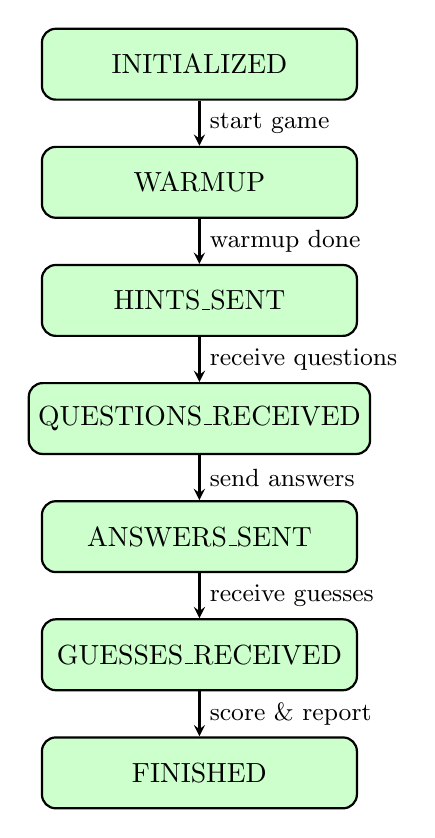
\begin{tikzpicture}[
    state/.style={draw, thick, fill=green!20, rounded corners=5pt, minimum width=4cm, minimum height=0.9cm, align=center},
    arrow/.style={->, thick, >=stealth}
]
    \node[state] (init) at (0,7) {INITIALIZED};
    \node[state] (warmup) at (0,5.5) {WARMUP};
    \node[state] (hints) at (0,4) {HINTS\_SENT};
    \node[state] (questions) at (0,2.5) {QUESTIONS\_RECEIVED};
    \node[state] (answers) at (0,1) {ANSWERS\_SENT};
    \node[state] (guesses) at (0,-0.5) {GUESSES\_RECEIVED};
    \node[state] (finished) at (0,-2) {FINISHED};

    \draw[arrow] (init) -- (warmup) node[midway, right, font=\small] {start game};
    \draw[arrow] (warmup) -- (hints) node[midway, right, font=\small] {warmup done};
    \draw[arrow] (hints) -- (questions) node[midway, right, font=\small] {receive questions};
    \draw[arrow] (questions) -- (answers) node[midway, right, font=\small] {send answers};
    \draw[arrow] (answers) -- (guesses) node[midway, right, font=\small] {receive guesses};
    \draw[arrow] (guesses) -- (finished) node[midway, right, font=\small] {score \& report};
\end{tikzpicture}
\end{english}
\caption{מכונת מצבים של משחק בודד}
\label{fig:game-state-machine}
\end{figure}

\hebrewsubsection{מכונת מצבים של סוכן שחקן}

סוכן השחקן עובר בין מצבים מוגדרים. כל מצב קובע אילו פעולות מותרות:

\begin{fancytable}{lHH}{מצבי סוכן השחקן}
\label{tab:player-lifecycle-states}
מצב & תיאור & פעולות מותרות \\
\en{UNREGISTERED} & הסוכן טרם נרשם & שליחת בקשת רישום \\
\en{REGISTERING} & ממתין לאישור רישום & המתנה לתגובה \\
\en{REGISTERED} & נרשם לליגה & המתנה להקצאות \\
\en{WAITING\_FOR\_GAME} & ממתין להזמנה & קבלת \en{GAME\_INVITATION} \\
\en{IN\_GAME} & פעיל במשחק & תגובה לשאלות, שליחת ניחוש \\
\en{PAUSED} & מושהה (שידור \en{PAUSE}) & המתנה ל-\en{CONTINUE} \\
\en{ERROR} & שגיאה התרחשה & ניסיון התאוששות \\
\end{fancytable}

\begin{figure}[htbp]
\centering
\begin{english}
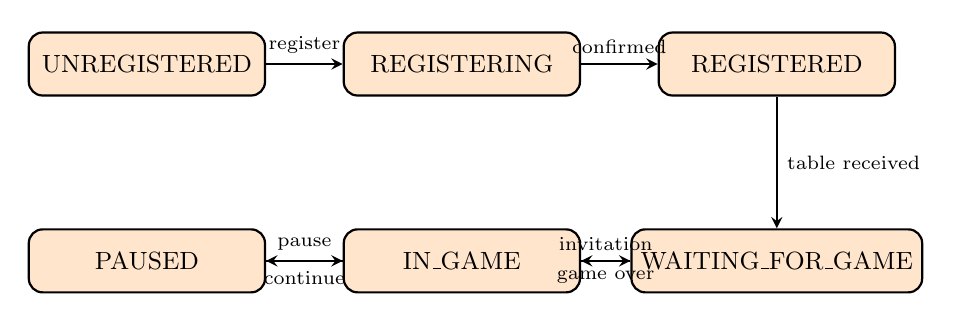
\begin{tikzpicture}[
    state/.style={draw, thick, fill=orange!20, rounded corners=5pt, minimum width=3cm, minimum height=0.8cm, align=center, font=\small},
    arrow/.style={->, thick, >=stealth}
]
    \node[state] (unreg) at (0,5) {UNREGISTERED};
    \node[state] (reging) at (4,5) {REGISTERING};
    \node[state] (regd) at (8,5) {REGISTERED};
    \node[state] (waiting) at (8,2.5) {WAITING\_FOR\_GAME};
    \node[state] (ingame) at (4,2.5) {IN\_GAME};
    \node[state] (paused) at (0,2.5) {PAUSED};

    \draw[arrow] (unreg) -- (reging) node[midway, above, font=\scriptsize] {register};
    \draw[arrow] (reging) -- (regd) node[midway, above, font=\scriptsize] {confirmed};
    \draw[arrow] (regd) -- (waiting) node[midway, right, font=\scriptsize] {table received};
    \draw[arrow] (waiting) -- (ingame) node[midway, above, font=\scriptsize] {invitation};
    \draw[arrow] (ingame) -- (waiting) node[midway, below, font=\scriptsize] {game over};
    \draw[arrow] (ingame) -- (paused) node[midway, above, font=\scriptsize] {pause};
    \draw[arrow] (paused) -- (ingame) node[midway, below, font=\scriptsize] {continue};
\end{tikzpicture}
\end{english}
\caption{מכונת מצבים של סוכן השחקן}
\label{fig:player-agent-state-machine}
\end{figure}

\hebrewsubsection{מכונת מצבים של סוכן שופט}

סוכן השופט מנהל את המשחק ואחראי על מספר שלבים נוספים:

\begin{fancytable}{lHH}{מצבי סוכן השופט}
\label{tab:referee-lifecycle-states}
מצב & תיאור & פעולות מותרות \\
\en{UNREGISTERED} & הסוכן טרם נרשם & שליחת בקשת רישום \\
\en{REGISTERED} & נרשם לליגה & המתנה להקצאות \\
\en{ASSIGNED} & הוקצה למשחק & שליחת הזמנות לשחקנים \\
\en{MANAGING\_GAME} & מנהל משחק פעיל & שליחת רמזים, קבלת שאלות \\
\en{SCORING} & מחשב ציונים & חישוב, שליחת משוב \\
\en{REPORTING} & מדווח תוצאות & שליחת \en{MATCH\_RESULT} \\
\en{PAUSED} & מושהה & המתנה ל-\en{CONTINUE} \\
\end{fancytable}

\begin{figure}[htbp]
\centering
\begin{english}
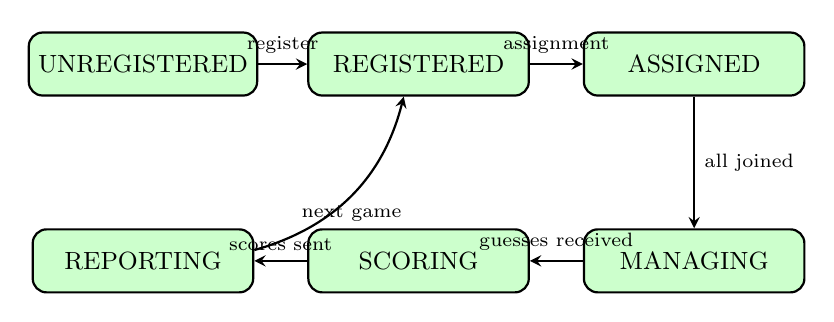
\begin{tikzpicture}[
    state/.style={draw, thick, fill=green!20, rounded corners=5pt, minimum width=2.8cm, minimum height=0.8cm, align=center, font=\small},
    arrow/.style={->, thick, >=stealth}
]
    \node[state] (unreg) at (0,4) {UNREGISTERED};
    \node[state] (regd) at (3.5,4) {REGISTERED};
    \node[state] (assigned) at (7,4) {ASSIGNED};
    \node[state] (managing) at (7,1.5) {MANAGING};
    \node[state] (scoring) at (3.5,1.5) {SCORING};
    \node[state] (reporting) at (0,1.5) {REPORTING};

    \draw[arrow] (unreg) -- (regd) node[midway, above, font=\scriptsize] {register};
    \draw[arrow] (regd) -- (assigned) node[midway, above, font=\scriptsize] {assignment};
    \draw[arrow] (assigned) -- (managing) node[midway, right, font=\scriptsize] {all joined};
    \draw[arrow] (managing) -- (scoring) node[midway, above, font=\scriptsize] {guesses received};
    \draw[arrow] (scoring) -- (reporting) node[midway, above, font=\scriptsize] {scores sent};
    \draw[arrow] (reporting) to[bend right=30] node[midway, below, font=\scriptsize] {next game} (regd);
\end{tikzpicture}
\end{english}
\caption{מכונת מצבים של סוכן השופט}
\label{fig:referee-agent-state-machine}
\end{figure}

% =============================================================================
\hebrewsection{טבלת הקצאת קבוצות משחק}
\label{sec:game-group-assignment}
% =============================================================================

\hebrewsubsection{סכמת הטבלה}

טבלה~\ref{tab:game-group-assignment-schema} מציגה את מבנה טבלת הקצאת קבוצות המשחק.

\begin{fancytable}{llH}{סכמת טבלת הקצאת קבוצות משחק}
\label{tab:game-group-assignment-schema}
שדה & סוג & תיאור \\
\en{season\_id} & \en{VARCHAR(3)} & מזהה העונה (\en{S01}, \en{S02}) \\
\en{round\_id} & \en{VARCHAR(2)} & מספר המחזור (\en{01}--\en{06}) \\
\en{game\_id} & \en{VARCHAR(7)} & מזהה משחק מורכב (\en{SSRRGGG}, למשל \en{0101001}) \\
\en{referee\_id} & \en{VARCHAR} & מזהה השופט (\en{R-Q21G-xxx}) \\
\en{player\_a\_id} & \en{VARCHAR} & מזהה שחקן א' (\en{P-Q21G-xxx}) \\
\en{player\_b\_id} & \en{VARCHAR} & מזהה שחקן ב' (\en{P-Q21G-xxx}) \\
\en{game\_status} & \en{ENUM} & מצב המשחק (אחד מחמישה) \\
\en{created\_at} & \en{TIMESTAMP} & זמן יצירת ההקצאה \\
\en{updated\_at} & \en{TIMESTAMP} & זמן עדכון אחרון \\
\end{fancytable}

\hebrewsubsection{מצבי המשחק (\en{game\_status})}

איור~\ref{fig:game-status-state-machine} מציג את מכונת המצבים של סטטוס המשחק.

\begin{figure}[htbp]
\centering
\begin{english}
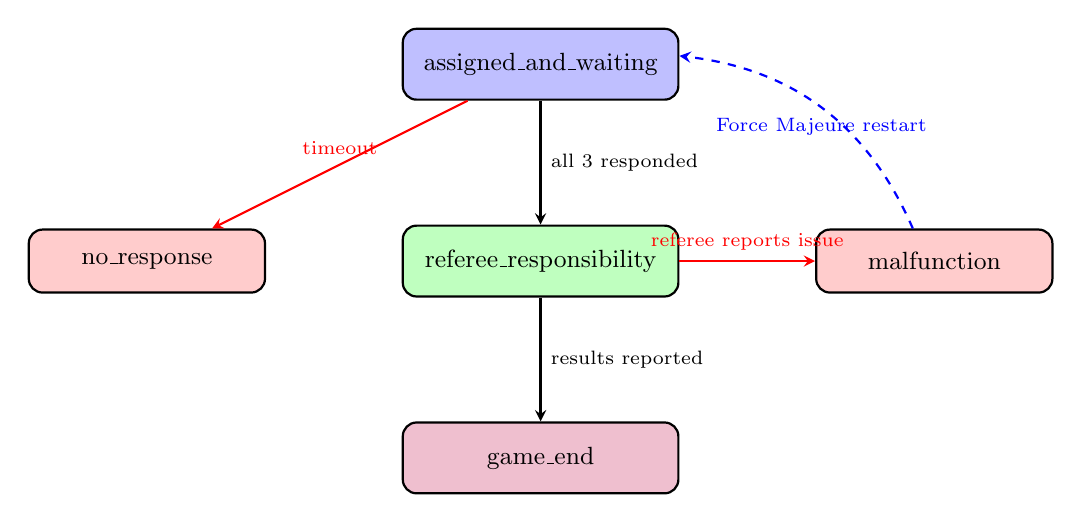
\begin{tikzpicture}[
    state/.style={draw, thick, fill=#1!25, rounded corners=5pt, minimum width=3.5cm, minimum height=0.9cm, align=center, font=\small},
    arrow/.style={->, thick, >=stealth},
    error/.style={draw, thick, fill=red!20, rounded corners=5pt, minimum width=3cm, minimum height=0.8cm, align=center, font=\small}
]
    % Main flow
    \node[state=blue] (assigned) at (0,5) {assigned\_and\_waiting};
    \node[state=green] (referee) at (0,2.5) {referee\_responsibility};
    \node[state=purple] (end) at (0,0) {game\_end};

    % Error states
    \node[error] (malfunction) at (5,2.5) {malfunction};
    \node[error] (noresponse) at (-5,2.5) {no\_response};

    % Main arrows
    \draw[arrow] (assigned) -- (referee) node[midway, right, font=\scriptsize] {all 3 responded};
    \draw[arrow] (referee) -- (end) node[midway, right, font=\scriptsize] {results reported};

    % Error arrows
    \draw[arrow, red] (referee) -- (malfunction) node[midway, above, font=\scriptsize] {referee reports issue};
    \draw[arrow, red] (assigned) -- (noresponse) node[midway, above, font=\scriptsize] {timeout};

    % Recovery
    \draw[arrow, dashed, blue] (malfunction) to[bend right=30] node[midway, below, font=\scriptsize] {Force Majeure restart} (assigned);

\end{tikzpicture}
\end{english}
\caption{מכונת מצבים של סטטוס המשחק --- חמישה מצבים אפשריים}
\label{fig:game-status-state-machine}
\end{figure}

\begin{fancytable}{lHH}{תיאור מצבי המשחק}
\label{tab:game-status-values}
מצב & תיאור & פעולה נדרשת \\
\en{assigned\_and\_waiting} & הודעת הקצאה נשלחה & ממתינים לתגובות \\
\en{referee\_responsibility} & כולם אישרו & השופט מנהל המשחק \\
\en{malfunction} & תקלה טכנית & בדיקת מנהל הליגה \\
\en{no\_response} & אין תגובה בזמן & הפסד טכני לחסר-התגובה \\
\en{game\_end} & המשחק הסתיים & תוצאות נרשמו בטבלה \\
\end{fancytable}

\hebrewsubsection{הבדל בין \en{malfunction} ל-\en{no\_response}}

\needspace{8\baselineskip}
\begin{notebox}[\hebtitle{הבחנה חשובה}]
\textbf{\en{malfunction}} --- השופט דיווח על תקלה טכנית במהלך המשחק (בעיית מערכת, כשל רשת וכו'). במקרה זה ניתן לבקש כוח עליון.

\textbf{\en{no\_response}} --- השופט לא הגיב כלל עד תום המחזור. במקרה זה השופט מקבל \num{0} נקודות ושני השחקנים מקבלים \num{2} נקודות כל אחד.
\end{notebox}

% =============================================================================
\hebrewsection{מודל הזהויות}
\label{sec:ids-model}
% =============================================================================

\hebrewsubsection{סוגי מזהים}

המערכת מגדירה מספר סוגי מזהים למעקב חד-משמעי:

\begin{fancytable}{lHlH}{סוגי מזהים במערכת}
\label{tab:system-ids-arch}
מזהה & סוג & דוגמה & תיאור \\
\en{league\_id} & מחרוזת & \en{Q21G\_2026} & מזהה ליגה ייחודי \\
\en{season\_id} & מחרוזת & \en{S01}, \en{S02} & מזהה עונה \\
\en{round\_id} & מחרוזת & \en{01}--\en{06} & מספר מחזור \\
\en{game\_id} & מחרוזת & \en{0101003} & מזהה משחק מורכב (\en{SSRRGGG}) \\
\en{player\_id} & מחרוזת & \en{P-Q21G-001} & מזהה שחקן \\
\en{referee\_id} & מחרוזת & \en{R-Q21G-001} & מזהה שופט \\
\en{message\_id} & \en{UUID} & \en{550e8400-...} & מזהה הודעה \\
\end{fancytable}

% =============================================================================
\hebrewsection{מערכת הניקוד המפורטת}
\label{sec:detailed-scoring}
% =============================================================================

\hebrewsubsection{ארבעת רכיבי הציון}

כל ניחוש של שחקן מוערך בארבעה רכיבים:

\textbf{\num{1}. דיוק משפט הפתיחה (\num{50}\%):}
\begin{itemize}
    \item התאמה לשונית --- מילים, סדר, מבנה
    \item התאמה קונספטואלית --- רעיון, תפקיד הפתיחה
    \item ציון גבוה להתאמה טובה, ביניים להתאמה חלקית
\end{itemize}

\textbf{\num{2}. נימוק המשפט (\num{20}\%):}
\begin{itemize}
    \item שימוש מושכל בתשובות שהתקבלו
    \item קישור הגיוני לתיאור הכללי
    \item עומק הבנה של תפקיד המשפט הפותח
\end{itemize}

\textbf{\num{3}. דיוק המילה האסוציאטיבית (\num{20}\%):}
\begin{itemize}
    \item התאמה למילה או לוריאציות קרובות
    \item אסוציאציה רחוקה או מתחום שגוי --- ציון נמוך
\end{itemize}

\textbf{\num{4}. נימוק האסוציאציה (\num{10}\%):}
\begin{itemize}
    \item קשר אינטליגנטי בין המילה לנושא הפסקה
    \item נימוק רדוד או מקרי --- ציון נמוך
\end{itemize}

\hebrewsubsection{חובת המשוב}

השופט מחויב להחזיר לכל שחקן:
\begin{itemize}
    \item הציון המספרי הכולל (\num{0}--\num{100})
    \item פירוט לכל אחד מארבעת הרכיבים
    \item הסבר קצר לכל רכיב
\end{itemize}

% =============================================================================
\hebrewsection{טיפול בשגיאות}
\label{sec:error-handling}
% =============================================================================

\hebrewsubsection{קודי שגיאה}

\begin{fancytable}{llHH}{קודי שגיאה עיקריים}
\label{tab:error-codes-arch}
קוד & שם & ניתן לניסיון חוזר & תיאור \\
\en{E001} & \en{TIMEOUT\_ERROR} & כן & תגובה לא התקבלה בזמן \\
\en{E005} & \en{NOT\_REGISTERED} & לא & סוכן לא רשום \\
\en{E009} & \en{CONNECTION\_ERROR} & כן & כשל רשת \\
\en{E011} & \en{AUTH\_MISSING} & לא & חסר אסימון אימות \\
\en{E012} & \en{AUTH\_INVALID} & לא & אסימון שגוי \\
\en{E020} & \en{MALFUNCTION\_REPORTED} & לא & השופט דיווח על תקלה \\
\en{E021} & \en{NO\_RESPONSE} & לא & אין תגובה עד תום מחזור \\
\en{E022} & \en{FORCE\_MAJEURE} & לא & כוח עליון --- משחק מבוטל \\
\end{fancytable}

\hebrewsubsection{מדיניות ניסיון חוזר}

מדיניות הניסיון החוזר מגדירה השהיה של \num{60} שניות בין ניסיונות במקרה של אי-קבלת תגובה. כלומר, אם נשלחה הודעה ולא התקבלה תגובה תוך \num{60} שניות, ניתן לשלוח בקשה נוספת. השהיה זו מתואמת עם מגבלות הקצב של \en{Gmail API} --- לפרטים נוספים על מגבלות השליחה וההמלצות למימוש ראו נספח~ה' (עמ'~\pageref{sec:gmail-api-limits}).

\begin{itemize}
    \item מספר ניסיונות מקסימלי: \num{3}
    \item השהיה בין ניסיונות: \num{60} שניות (במקרה של אי-תגובה)
    \item לאחר מיצוי ניסיונות: הפסד טכני
\end{itemize}

במידה והשופט אישר הערכה או ביצע ניסיונות, כל משך הזמנים של המשחק מתארך בהתאם. כלומר אם רק בניסיון השלישי הצליח הקשר, אזי משך המשחק הכולל הופך להיות במקום \num{15} דקות למשחק לכדי \num{18} דקות. שימו לב שהספירה של \num{3} ניסיונות היא אחידה לכל שחקן במשך כל המשחק שהשופט מנהל. כלומר לכל אחד מהמשתתפים יש עד \num{3} ניסיונות חוזרים, כלומר בסה"כ יש \num{9} ניסיונות חוזרים במשחק, מה שאומר שבמקרה הגרוע המשחק יכול להימשך עד תוספת זמן של \num{9} דקות למשחק.

\begin{warningbox}[\hebtitle{מגבלת הערכות מצטברות}]
שימו לב כי לא ניתן לאשר הערכות מצטברות של כלל הסוכנים במשחק מעבר ל-\num{10} דקות בכל המשחק. כלומר אם יש השהייה מכל סיבה, בין שבגין חוסר תגובה, ובין שבגין תקלה ובגין כל סיבה אחרת --- השופט לא יכול לאשר הערכה של יותר מ-\num{10} דקות במצטבר. \textbf{מודגש:} השופט חייב לאשר בקשה להערכה ובלבד שהתקבלה בהתאם להנחיות.
\end{warningbox}

\needspace{8\baselineskip}
\begin{notebox}[\hebtitle{הודעות מנהל הליגה}]
שימו לב שמנהל הליגה יכול לאשר הערכה גורפת. הסוכנים שלכם צריכים לדעת לקבל את הודעת מנהל הליגה ולשנות את לוחות הזמנים בהתאם להודעת מנהל הליגה. למשל, מנהל הליגה יכול להודיע כי משחק מסוים או מחזור משחקים מקבלים חלון זמנים חדש, ובמקרה כזה המשחקים שקיבלו ממנהל הליגה חלון זמן מתאפסים ומתקיימים מחדש. יש להכין את הסוכנים בהתאם. בזמן חלונות הזמן של החימום יתאפשר להתאמן בנושא מול מנהל הליגה.
\end{notebox}

% =============================================================================
\hebrewsection{סיכום}
% =============================================================================

פרק זה הציג את ארכיטקטורת מערכת הליגה:

\begin{itemize}
    \item ארכיטקטורת שלוש שכבות: ליגה, שיפוט, וחוקי משחק
    \item שלושה סוגי סוכנים: מנהל ליגה, שופט, ושחקן
    \item שרת הלוג מקבל \en{CC} של כל הודעות המשחק (ניתוח כמותי בנספח~ה')
    \item מכונות מצבים מוגדרות למשחק ולסוכן
    \item טבלת הקצאת קבוצות משחק עם חמישה מצבים אפשריים
    \item הבחנה בין \en{malfunction} (תקלה מדווחת) ל-\en{no\_response} (אי-תגובה)
    \item מודל זהויות עם מזהים ייחודיים למעקב
    \item מערכת ניקוד מפורטת עם ארבעה רכיבים
\end{itemize}

בפרק הבא נעמיק בפרוטוקול התקשורת המפורט בין הסוכנים.

\end{document}
